\documentclass[12pt,a4paper]{article}
\usepackage[utf8]{inputenc}
\usepackage{amssymb, amsmath, multicol}
\usepackage[english,russian]{babel}
\usepackage{graphicx}
\usepackage[shortcuts,cyremdash]{extdash}
\usepackage{wrapfig}
\usepackage{floatflt}
\usepackage{lipsum}
\usepackage{concmath}
\usepackage{euler}
\usepackage{tikz}  
\usetikzlibrary{graphs}
\usepackage{mathtext} 


\oddsidemargin=-15.4mm
\textwidth=190mm
\headheight=-32.4mm     
\textheight=277mm
\tolerance=100
\parindent=0pt
\parskip=8pt
%\pagestyle{empty}
\renewcommand{\tg}{\mathop{\mathrm{tg}}\nolimits}
\renewcommand{\ctg}{\mathop{\mathrm{ctg}}\nolimits}
\renewcommand{\arctan}{\mathop{\mathrm{arctg}}\nolimits}
\newcommand{\divisible}{\mathop{\raisebox{-2pt}{\vdots}}}

\graphicspath{{pictures/}}

\begin{document}
    \begin{center}
        Лабораторная работа 2.1.6.
        \\
        "Эффект Джоуля~---~Томсона"
        \\
        Радькин Кирилл Б01~---~005
    \end{center}
    Эффектом Джоуля~---~Томсона называется изменение температуры газа, медленно протекающего из области высокого давления в область низкого давления в условиях хорошей тепловой изоляции. В разряженных газах, которые приближаются по своим свойствам к идеальному газу, при таком течении температура не изменяется. Эффект Джоуля~---~Томсона демонстрирует отличие исследуемого газа от реального.\\\\
    В работе исследуется изменение температуры углекислого газа при медленном его течении по трубке с пористой перегородкой. Трубка хорошо теплоизолирована. Газ из области повышенного давления $P_1$ проходит через множество узких и длинных каналов пористой перегородки в область с атмосферным давлением $P_2$. Перепад давления $\Delta P = P_1 - P_2$ из-за большого сопротивления каналов может быть заметным даже при малой скорости течения газа в трубке. Величина эффекта Джоуля–Томсона определяется по разности температуры газа до и после перегородки. \\
    
    Рассмотрим стационарный поток газа между произвольными сечениями трубки (до перегородки и после нее). Пусть, для определенности, через трубку прошел 1 моль углекислого газа; $\mu$ — его молярная масса. Молярные объемы газа, его давления и отнесенные к молю внутренние энергии газа в сечениях $I$ и $II$ обозначим соответственно $V_1 , P_1 , U_1$ и $V_2 , P_2 , U_2$. Для того чтобы ввести в трубку объем $V_1$ , над газом нужно совершить работу $A_1 = P_1 V_1$. Проходя через сечение $II$, газ сам совершает работу $A_2 = P_2V_2$. Так как через боковые стенки не происходит ни обмена теплом, ни передачи механической энергии, то
    \begin{equation}
    	A_1 - A_2 = \left( U_2 + \dfrac{\mu v_2^2}{2}\right) - \left( U_1 + \dfrac{\mu v_1^2}{2} \right)
	\end{equation} 
    В уравнении ($1$) учтено изменение как внутренней (первые члены в скобках), так и кинетической (вторые члены в скобках) энергии газа. Подставляя в ($1$) написанные выражения для $A_1$ и $A_2$ и перегруппировывая члены, найдем
    \begin{equation}
    H_1 - H_2 = \left( U_1 + P_1V_1 \right) - \left( U_2 + P_2V_2 \right) = \dfrac{\mu \left( v_2^2 - v_1^2 \right)}{2}
    \end{equation}
    Сделаем несколько замечаний. Прежде всего отметим, что в процессе Джоуля–Томсона газ испытывает в пористой перегородке существенное трение, приводящее к ее нагреву. Потери энергии на нагрев трубки в начале процесса могут быть очень существенными и сильно
искажают ход явления. После того как температура трубки установится и газ станет уносить с собой все выделенное им в пробке тепло, формула ($1$) становится точной, если, конечно, теплоизоляция трубки достаточно хороша и не происходит утечек тепла наружу через ее
стенки.\\

	Второе замечание связано с правой частью ($2$). Процесс Джоуля–Томсона в чистом виде осуществляется лишь в том случае, если правой частью можно пренебречь, т. е. если макроскопическая скорость газа с обеих сторон трубки достаточно мала. У нас сейчас
нет критерия, который позволил бы установить, когда это можно сделать. Поэтому мы отложим на некоторое время обсуждение вопроса о правой части ($2$), а пока будем считать, что энтальпия газа не меняется.
	\begin{equation}
	\mu = \dfrac{\Delta T}{\Delta P} \approx \dfrac{2a/RT - b}{C_p} 
	\end{equation}
	Из формулы ($3$) видно, что эффект Джоуля–Томсона для не очень плотного газа зависит от соотношения величин $a$ и $b$, которые оказывают противоположное влияние на знак эффекта. Если силы взаимодействия между молекулами велики, так что превалирует «поправка на давление», то основную роль играет член, содержащий a, и
	\begin{equation*}
	\dfrac{\Delta T}{\Delta P} > 0
	\end{equation*}
	т. е. газ при расширении охлаждается ($\Delta T$ < 0, так как всегда $\Delta P$ < 0). В обратном случае (малые $a$):
	\begin{equation*}
	\dfrac{\Delta T}{\Delta P} < 0
	\end{equation*}
	т. е. газ нагревается ($\Delta T$ > 0, так как по-прежнему $\Delta P$ < 0). \\
	
	Этот результат нетрудно понять из энергетических соображений. Как мы уже знаем, у идеального газа эффект Джоуля–Томсона отсутствует. Идеальный газ отличается от реального тем, что в нем можно пренебречь потенциальной энергией взаимодействия молекул. Наличие этой энергии приводит к охлаждению или нагреванию реальных газов при расширении. При больших a велика энергия притяжения молекул. Это означает, что потенциальная энергия молекул при их
сближении уменьшается, а при удалении — при расширении газа —возрастает. Возрастание потенциальной энергии молекул происходит за счет их кинетической энергии — температура газа при расширении падает. Аналогичные рассуждения позволяют понять, почему расширяющийся газ нагревается при больших значениях $b$.При температуре $T_i $ коэффициент $\mu$ обращается в нуль. Используя связь между коэффициентами $a$ и $b$ и критической температурой:
	\begin{equation}
	T_i = \dfrac{27}{4}T_k
	\end{equation}
	При температуре $T_i$ эффект Джоуля–Томсона меняет знак: ниже температуры инверсии эффект положителен ($\mu > 0$, газ охлаждается), выше $T_i$ эффект отрицателен ($\mu < 0$, газ нагревается). \\
	
	Температура инверсии у всех газов лежит значительно выше критической. Для большинства газов $\dfrac{T_i}{T_k} = 5 - 8$. Например, для гелия $T_i$ = 46 K, $T_k$ = 5,2 К; для водорода $T_i$ = 205 К, $T_k$ = 33 К; для азота $T_i$ = 604 К, $T_k$ = 126 К; для воздуха $T_i$ = 650 К, $T_k$ = 132,6 К; для углекислого газа $T_i$ = 2050 К, $T_k$ = 304 К. Температура инверсии у гелия и водорода значительно ниже комнатной, поэтому при обычных температурах эти газы при расширении нагреваются. Температура инверсии остальных газов выше комнатной, и при нормальных условиях температура при расширении газа падает.\\
	
	Сравнивая приведенные значения T инв и T кр , можно убедиться в том, что предсказания, следующие из формулы Ван-дер-Ваальса, у реальных газов выполняются не очень хорошо. Правильно передавая качественную картину поведения реальных газов, формула Ван-дер-Ваальса не претендует на хорошее количественное описание этой картины.\\
	
    Экспериментальная установка: \\
    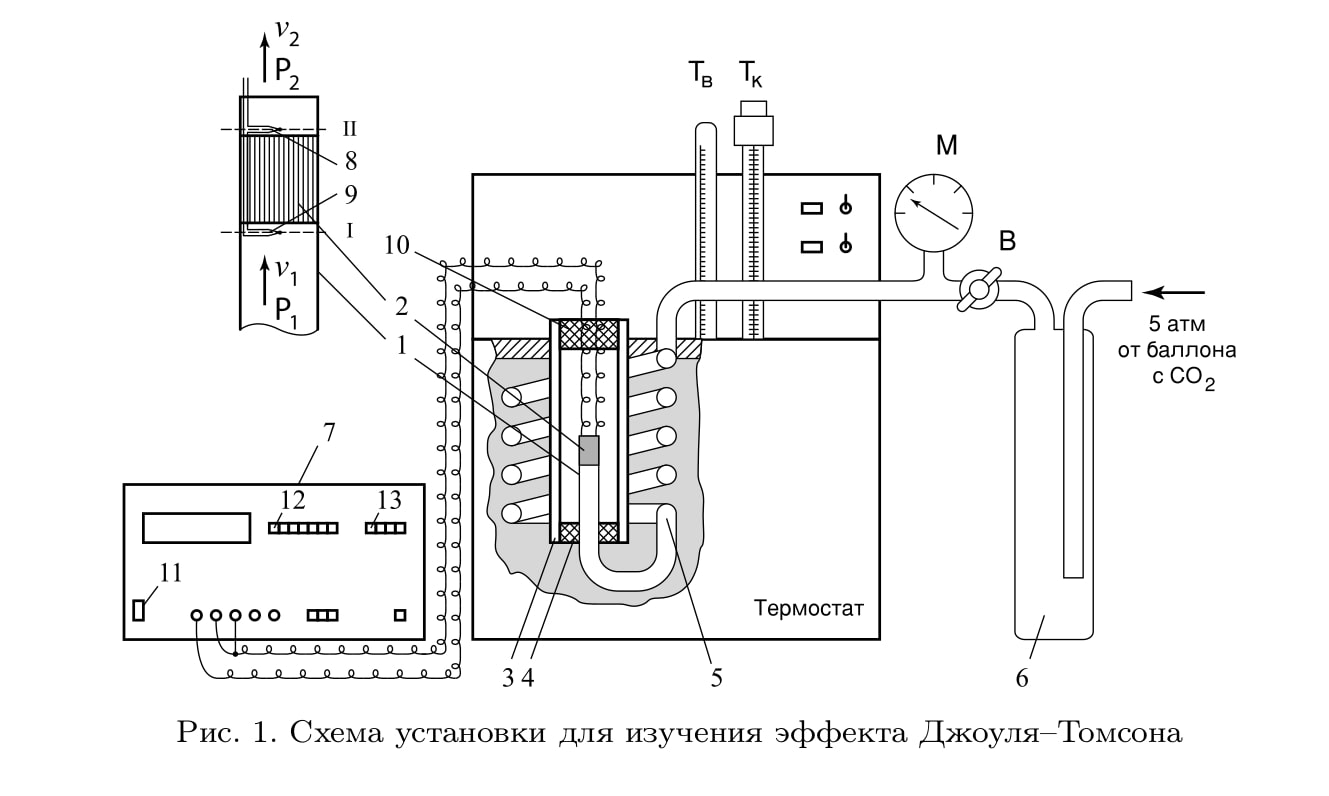
\includegraphics[scale=0.4]{ust.jpg}\\\\
    В работе исследуется изменение температуры углекислого газа при медленно его стекании по трубке с пористой перегородкой. \\\\
    Ход работы: \\
	1) Настроим вольтметр и термостат. \\\\
	2) Измерим показания вольметра при $\Delta P = 0$. Используем это значение для дальнейшей корректировки показаний: $E = U(\Delta P) - U(0)$. \\\\
	3) Откроем регулирующий вентиль настолько, чтобы избыточное давление составило $\Delta P \approx4$~атм.\\\\
	4) Через 10~---~15 минут (когда установятся все переходные процессы), запишем показания вольтметра. \\\\
	5) При помощи вентиля уменьшим давление на $0.5$ атм. Через 5 минут, когда установятся давление и разность температур, снова запишем показания вольтметра. \\\\
	6) Проведем измерения для нескольких значений давления , $T = 20^{\circ}C$.\\\\
	\begin{tabular}{c | c | c | c | c | c}
		$\Delta P$, атм. & $4$ & $3.5$ & $3$ & $2.5$ & $2$ \\ \hline
		$V$, мкв. & $134$ & $120$ & $98$ & $76$ & $57$ \\
	\end{tabular}\\\\
	7) $T = 30^{\circ}C$\\\\
	\begin{tabular}{c | c | c | c | c | c}
		$\Delta P$, атм. & $4$ & $3.5$ & $3$ & $2.5$ & $2$ \\ \hline
		$V$, мкв. & $130$ & $112$ & $93$ & $74$ & $54$ \\
	\end{tabular}\\\\
	8) $T = 50^{\circ}C$\\\\
	\begin{tabular}{c | c | c | c | c | c}
		$\Delta P$, атм. & $4$ & $3.5$ & $3$ & $2.5$ & $2$ \\ \hline
		$V$, мкв. & $115$ & $101$ & $81$ & $66$ & $53$ \\
	\end{tabular}\\\\
	9) Чтобы из показаний вольметра получить разность температур, необходимо разделить их на чувствительность термопары: $40.7$ мкВ/$^{\circ}C$ для температуры $T = 20^{\circ}C$, $41.6$ мкВ/$^{\circ}C$ для $T = 30^{\circ}C$, $43.3$ мкВ/$^{\circ}C$ для $T = 50^{\circ}C$\\\\
	10) Построим график зависимости $\Delta T$ от $\Delta P$ для различных $T$:\\\\
	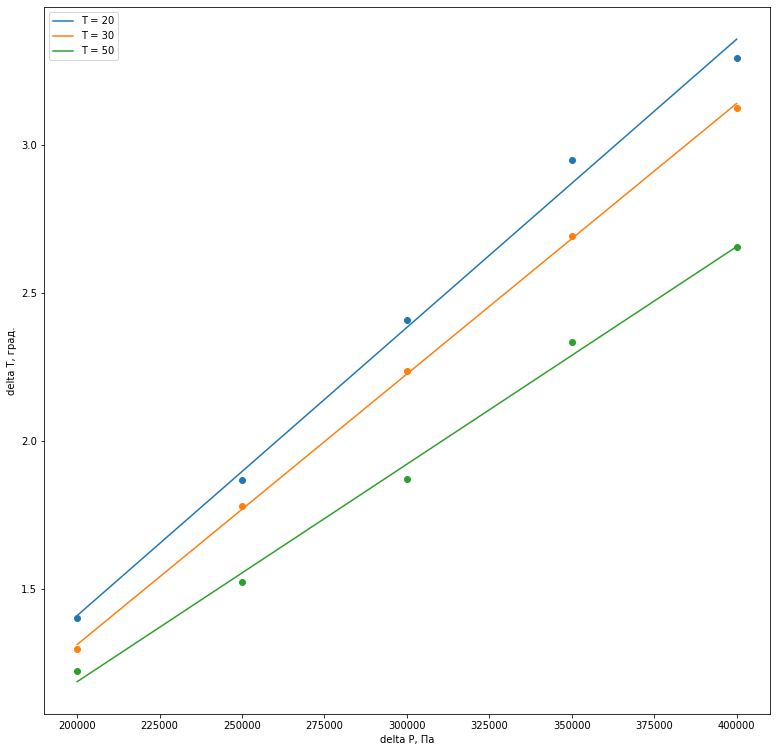
\includegraphics[scale=0.6]{graph.png} \\\\
	Коэффициенты Джоуля-Томсона:
	\begin{itemize}
		\item $T = 20^\circ C$: $\mu = (97.3 \pm 3.1) \cdot 10^{-7}$ К/Па
		\item $T = 30^\circ C$: $\mu = (91.3 \pm 0.7) \cdot 10^{-7}$ К/Па
		\item $T = 50^\circ C$: $\mu = (73.4 \pm 2.3) \cdot 10^{-7}$ К/Па
	\end{itemize}
	11) Используя формулу $\dfrac{\Delta T}{\Delta P} = \dfrac{(2a/RT - b}{C_p}$ и экспериментальные данные, определим постоянные $a$ и $b$ для двух пар температур:$T = 20^{\circ}C$ и $T = 30^{\circ}C$ и $T = 30^{\circ}C$ и $T = 50^{\circ}C$:
	\begin{itemize}
		\item Для $T = 20^{\circ}C$ и $T = 30^{\circ}C$: $a = 0.9$ Н * м$^4$/моль, $b = 34 \cdot 10^{-5}$ м$^3$/моль.
		\item Для $T = 30^{\circ}C$ и $T = 50^{\circ}C$: $a = 1.5$ Н * м$^4$/моль, $b = 81 \cdot 10^{-5}$ м$^3$/моль.
	\end{itemize}
	Табличные $a$ и $b$:
	\begin{itemize}
		\item $a = 0.37$ Н * м$^4$/моль
		\item $b = 4.5 \cdot 10^{-5}$ м$^3$/моль 
	\end{itemize}
	12) Используя найденные постоянные, посчитаем $T_{inv} = \dfrac{2a}{Rb}$:
	\begin{itemize}
		\item Для $T = 20^{\circ}C$ и $T = 30^{\circ}C$: $T_{inv} = 636 \pm 25K$
		\item Для $T = 30^{\circ}C$ и $T = 50^{\circ}C$: $T_{inv} = 442 \pm 17K$
	\end{itemize}
	Вывод: настоящая $T_{inv} = 2050 K$ (для углекислого газа) и коэффициенты $a$ и $b$ не совпадает с полученными нами значениеми, что говорит о неточности и неприменимости уравнения Ван-дер-Вальса для идеального газа.
\end{document}